\documentclass[tikz]{standalone}

\usepackage{fontspec}

\usetikzlibrary{arrows}
\usetikzlibrary{calc}
\usetikzlibrary{decorations.pathreplacing}
\usetikzlibrary{positioning}
\usetikzlibrary{matrix}

\usepackage{fontspec}

\begin{document}

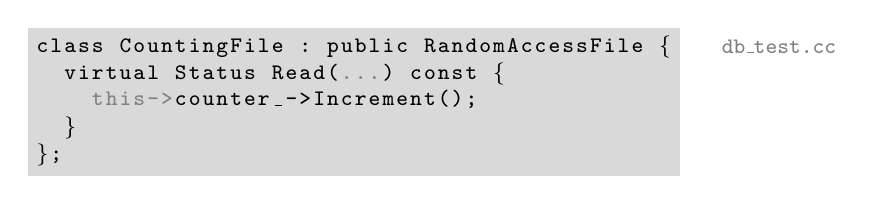
\begin{tikzpicture}
  [node distance=5mm, >=stealth',
  every node/.style={font=\footnotesize},
  every matrix/.style={fill=black!15, inner sep=1mm, row sep=0.5mm,
                        matrix of nodes, nodes in empty cells,
                        minimum height=0.5em, minimum width=.5em,
                        nodes={anchor=base, inner sep=0, font=\ttfamily\footnotesize}}]

  \matrix (snippet) {
c & l & a & s & s &   & C & o & u & n & t & i & n & g & F & i & l & e &   & : &   & p & u & b & l & i & c &   & R & a & n & d & o & m & A & c & c & e & s & s & F & i & l & e &   & \{ \\
  &   & v & i & r & t & u & a & l &   & S & t & a & t & u & s &   & R & e & a & d & ( & |[black!50]|. & |[black!50]|. & |[black!50]|. & ) &   & c & o & n & s & t &   & \{ &   &   &   &   &   &   &   &   &   &   &   &   \\
  &   &   &   & |[black!50]|t & |[black!50]|h & |[black!50]|i & |[black!50]|s & |[black!50]|- & |[black!50]|> & c & o & u & n & t & e & r & \_ & - & > & I & n & c & r & e & m & e & n & t & ( & ) & ; &   &   &   &   &   &   &   &   &   &   &   &   &   &   \\
  &   & \} &   &   &   &   &   &   &   &   &   &   &   &   &   &   &   &   &   &   &   &   &   &   &   &   &   &   &   &   &   &   &   &   &   &   &   &   &   &   &   &   &   &   &   \\
\} & ; &   &   &   &   &   &   &   &   &   &   &   &   &   &   &   &   &   &   &   &   &   &   &   &   &   &   &   &   &   &   &   &   &   &   &   &   &   &   &   &   &   &   &   &   \\
  };

 \node [above, anchor=west, black!50, xshift=0.5cm]
        at (snippet-1-46.east)
        {\texttt{db\_test.cc}};
\end{tikzpicture}

\end{document}
